\subsection{Overview}
The architecture of the S2B is a distributed client-server architectural design, structured according to three logic layers:
\begin{itemize}
	\item \textbf{Presentation level P}: manages the user interaction with the system. This layer contains the interfaces able to provide the functions of the application to the users.\\
	To the presentation layer belong the web app, the phone application and the software on the ticket printer and on the QR reader.
	\item \textbf{Business logic or Application layer (A)}: handles the business logic of the application and its functionalities. This layer represent the core of the application logic.
	\item \textbf{Data access layer (D)}: manages information and data, by accessing the database.  
\end{itemize}
Every logic layer can be mapped in an hardware layer.\\
The presentation layer is composed by the smartphone or the computer of the user, the ticket printer outside the stores, the QR reader and the turnstiles.\\
The application layer is composed by the application server.
The data layer is composed by the database server.\\\\\\
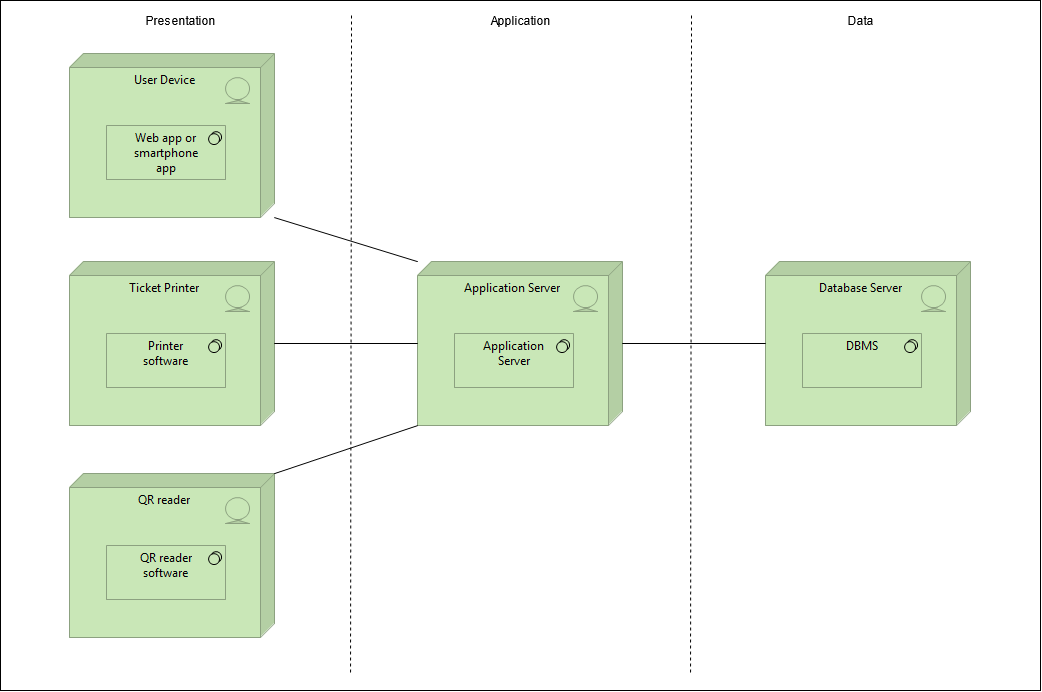
\includegraphics[scale=0.4]{Images/Archimate.png}\\
This image shows the high level representation of the three-layer architecture, where we have all the devices used to interact with the user and their respective software, that have to connect to the application server, which is able to communicate with the database server.\\
Although very simple, this high level view shows how a three tier architecture can provide more flexibility to the system, splitting the server side in two logical layers. It is also very useful from a security viewpoint: in fact the data are kept separated from the user by the application layer, so that all sensitive information are protected from undesired access.
\newpage
Let us now have a more in-depth look at the system architecture.\\\\
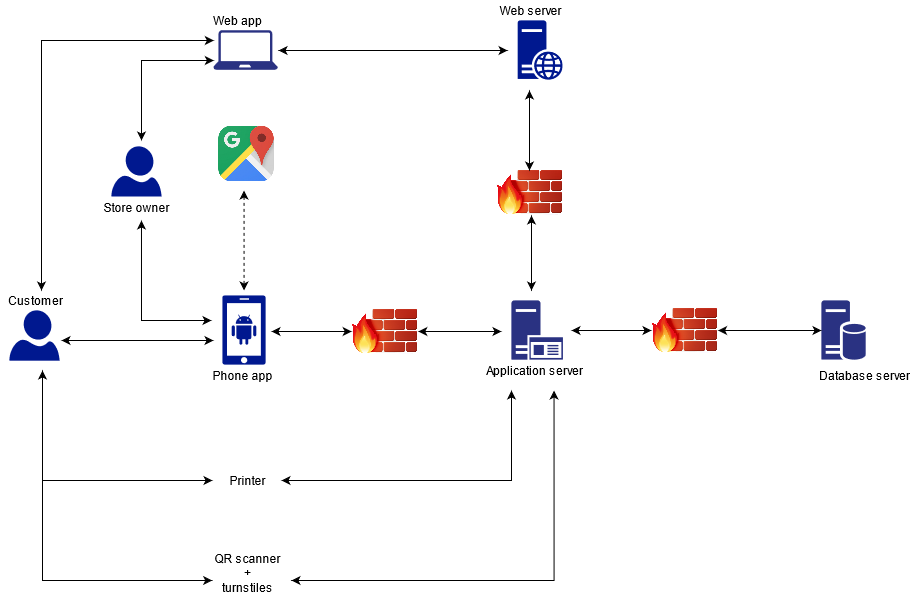
\includegraphics[scale=0.5]{Images/System Architecture.png}\\\\
Here we can better see how each tier of the previously defined architecture is mapped in the system. The customer is capable to interact with the system in several ways: through the phone app on his smartphone, by the web app on his computer, using the printer outside the store (in order to create an on premise reservation) or via QR scanner, which unlocks the turnstiles and validate enter and exit from the store. In order to provide an estimation of the travel time from the location of the customer to the store, the system uses the GPS technology through the Google Maps API.\\
The store owner, from his/her side, can only access the system from the web app or the phone application; this is because in the role of owner he/she does not need to access the market, and use the system only to control occupation and statistics of the stores.\\
The web app does not communicate directly with the application server, but must traverse the web server, which provide the web pages to the browser.\\
The application and web servers ere protected from the outside by a first firewall, which creates a demilitarized zone for them. Then, the application server communicates with the database server, which contains the database management system, through a second and more restrictive firewall, that isolate the database from possible attacks. This double firewall ensures the security properties for the system.\\
In order to create reservations, the clients must communicate synchronously with the server, as they have no information on the queue. The application server, then communicates synchronously with the database server to retrieve information or asynchronously to store information when needed.\\
In the image above the server element must not be considered as a single machine: if so the architecture would be poorly scalable, and heavy traffic would make the system crash. To guarantee scalability we use a node replication approach, which involves the use of a node balancer which redirect the traffic between multiple servers.\newpage
\begin{figure}[h]
	\noindent
	\makebox[\textwidth]{
	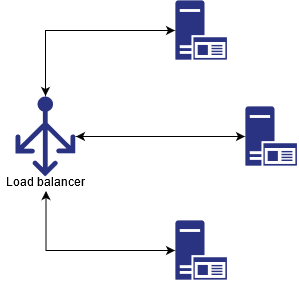
\includegraphics[scale=0.5]{Images/LoadBalancer.png}}
\end{figure}
This image show an example of how this method works for the application tier: in this case the load balancer splits the work between three application servers, but of course there might be more. Moreover this approach is used also for the web server and the database server, according to the needs of the system.\\
Until now we have used an informal view of the architecture; in the next sections we will keep deepening the architecture and its characteristics.\newpage
\subsection{Component View}
Here we display the main component architecture of our S2B. Since the ApplicationServer contains all the business logic, we will describe in detail the structure of its subcomponents.\\\\
\begin{figure}[H]
	\noindent
	\makebox[\textwidth]{
	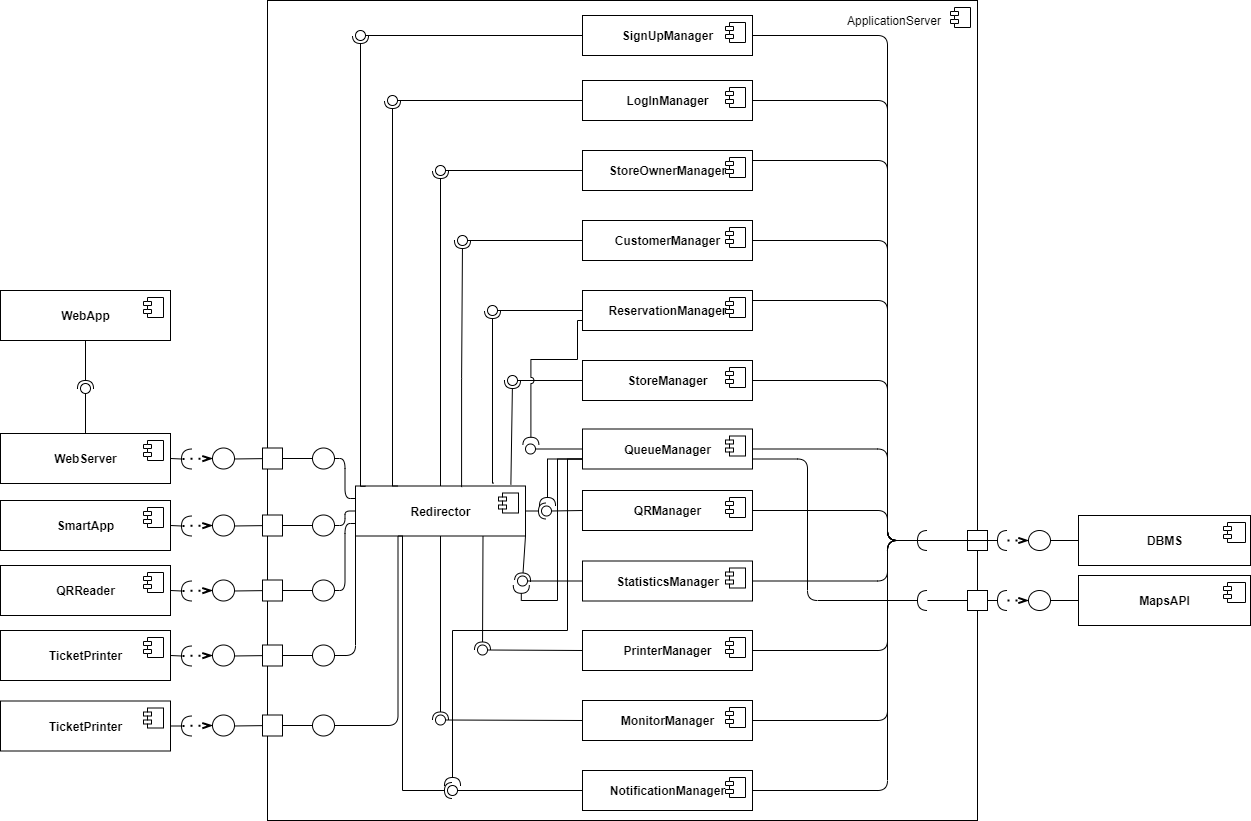
\includegraphics[scale=0.35]{Images/Component.png}}
\end{figure}


\subsubsection{WebApp}
This component allows customer and store owners to access their respective services on a computer. It requires a WebServer.
\subsubsection{WebServer}
This component communicates directly with the ApplicationServer and serves web pages to implement the WebApp component.
\subsubsection{SmartApp}
This component allows customers and store owners to access their respective services on a smartphone, by interfacing with the ApplicationServer. It is composed of the following subcomponents:
\paragraph{StoreOwnerService}Allows the store owner to access the functionalities that the system reserved to him/her.
\paragraph{CustomerService}Allows the customer to access the functionalities that the system reserved to him/her.
\paragraph{NotificationService}Periodically receives the waiting time from the NotificationManager and calls MapsAPI to get the time to reach the store from the current position and if it is greater or equal to the waiting time (plus a constant, to give a little notice to the customer) it notifies the customer.
\subsubsection{QRReader}
This component reads user provided QRCodes and sends them to the ApplicationServer, thus enabling authentication for turnstiles.
\subsubsection{TicketPrinter}
This component accepts a user document and after having validated it through the ApplicationServer, it prints a reservation ticket with a QR.
\subsubsection{StoreMonitor}
This component updates periodically calling the ApplicationServer, which provides it with the number of the last authorized reservation, thus notifying customers in front of the store when they can enter.
\subsubsection{Redirector}
This component provides an external interface for the previously described components, and allows them to communicate with the components that are located within the ApplicationServer, that we describe below.
\subsubsection{AccessManager}
This component allows users to connect to the services, via sign up and login.
\paragraph{SignupManager}
This component allows customers and store owners that provide a valid identification document to register to the service, thus gaining access to its functionalities, provided that they log in. It is called through WebApp or SmartApp, and needs to access the DBMS to search for existing users with same identification document (to avoid duplication), and to create a new user.
\paragraph{LoginManager}
This component allows customers and store owners to log in the service, thus gaining access to its functionalities. It is called by WebApp and SmartApp components, and needs to access the DBMS to verify user credentials against the stored ones.
\subsubsection{UserManager}
This component allows users to change their profile.
\paragraph{StoreOwnerManager}
This component is accessed through WebApp or SmartApp and allows store owners to edit their credentials (obtained during sign up process), thus it needs access to DBMS.
\paragraph{CustomerManager}
This component is accessed through WebApp or SmartApp and allows customers to edit their credentials (obtained during sign up process), thus it needs access to DBMS.
\subsubsection{ReservationManager}
This component is accessed through WebApp or SmartApp by customers and allows them to send a reservation for a specific store, to delete an existing reservation, or to view status of non expired reservations (QR code, position in queue, status) by accessing QueueManager. It needs to access DBMS to retireve the list of the departments of the store that the reservation targets and, in case of an immediate reservation, to verify that the store is open at the current time. It needs access to DBMS also to fetch the list of user reservation along with their information, and to delete them if required. Whenever a customer creates a reservation it is saved into the database. This component is also accessed by the TicketPrinter whenever a customer creates an on premise reservation.
\subsubsection{StoreManager}
This component is accessed through WebApp or SmartApp, and allows store owners to view owned stores, add new stores, delete existing stores or update information of existing stores, such as the list of departments and their respective maximum occupation. It needs to access the DBMS to execute the previous functions.
\subsubsection{QueueManager}
This component contains the information about the people that are currently waiting to enter the store and those that are already inside it.\\
It is accessed by the ReservationManager to add or remove a reservation from a queue of a specific store.
It is also accessed by the QRManager whenever an authorized customer wants to view the QR and when he/she enters or exits the store.
Moreover it accesses MonitorManager every time the number of the last authorized reservation of a store changes.
Finally it is accessed by NotificationManager in order to get the list of the customers currently waiting.\\
It needs access to DBMS to update the status of each reservation and entry and exit times. It checks periodically the number of customers currently present and the maximum occupation for every store and computes an estimated time that customers have to wait before gaining authorization to enter a specific store if such store has already reached maximum occupation.\\
This component accesses StatisticsManager to improve the computation of the time a customer needs to wait before being authorized to enter the store.
\subsubsection{QRManager}
This component accesses QueueManager whenever a customer needs to view a QR for a reservation: if a QR has already been generated for that reservation it is returned to QRManager, otherwise it is generated by QRManager and sent to QueueManager. When QRReader reads a QR code from a customer it calls QRManager, that accesses QueueManager to check that the reservation is existing and authorized, and if so it send the entry/exit time to the QueueManager and returns the QRReader the permission to unlock turnstile.
\subsubsection{StatisticsManager}
This component is accessed by QueueManager to improve the estimate of the time that a customer needs to wait before being authorized to enter a specific store. This component is accessed by a store owner through WebApp or SmartApp to visualize statistics. This component accesses the DBMS periodically to obtain the data with which to generate the statistics, and to save such statistics.
\subsubsection{PrinterManager}
This component allows the store owner with WebApp or SmartApp to register a TicketPrinter. This component also allows customer identification through TicketPrinter by validating a provided identification document. This component needs to access the DBMS to register or unregister instances of TicketPrinter.
\subsubsection{MonitorManager}
This component allows to update periodically a StoreMonitor. It is updated by the QueueManager every time the number of the last authorized reservation of a store changes, and then updates all the StoreMonitor registered for that store.
\subsubsection{NotificationManager}
This component accesses the NotificationService to provide the wait time. This component periodically accesses the QueueManager to get this information.
\subsubsection{MapsAPI}
This component accesses an external mapping service (i.e. GoogleMaps) to compute the estimated time to reach the store from the current position of the device with the selected means of transport.
\subsubsection{DBMS}
This component is the DataBase Management System accessed by the ApplicationServer to perform create/read/update/delete operations on the DB.
\subsubsection{Additional specification}
For what concerns the smartphone application, it is a thick client: in fact beside the presentation logic, it contains a small part of the application logic. Indeed, the phone app can check the validity of the information inserted by the user when creating a reservation and, more importantly, it checks when it is time to notify the customer about its turn to reach the store, based on the position of the device and the position of the store (received by the server). It is important that the phone app does this computations, because the position of the customer, necessary to know how long will it take to go to the market, can only be detected by the end device.\\
The web app, of course, is instead a thin client, because, being it a browser application, will only work on the presentation logic, to show the interface to the user.\\
In order to guarantee the reliability of the system, both the web servers and the application servers must be replicated, so that in case of one of them goes down the application can still work.\\
The load balancer, that in one of the previous diagram has been represented as a single component, may become overloaded by the requests. To prevent this it must be replicated too.\\
To optimize the routing process we can divide the redirector in several subcomponents, one for each of the possible devices that will use it.\\
\begin{figure}[H]
	\noindent
	\makebox[\textwidth]{
	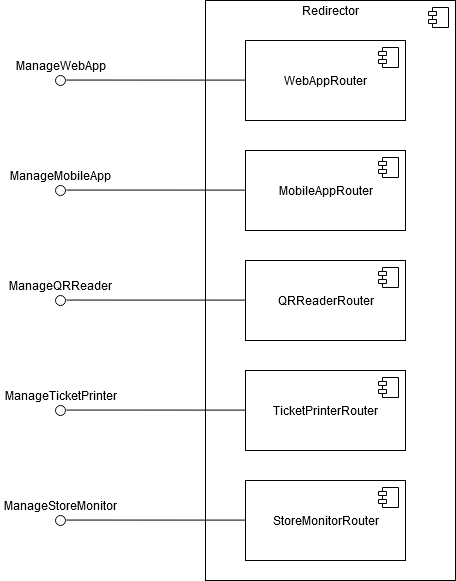
\includegraphics[scale=0.40]{Images/RedirectorExpanded.png}}
\end{figure}
This image shows how each interface connects with the redirector's subcomponents. Of course, each of them will provide a different routing on the possible interfaces of the system, as shown in the following diagrams.\\
\begin{figure}[H]
	\noindent
	\makebox[\textwidth]{
	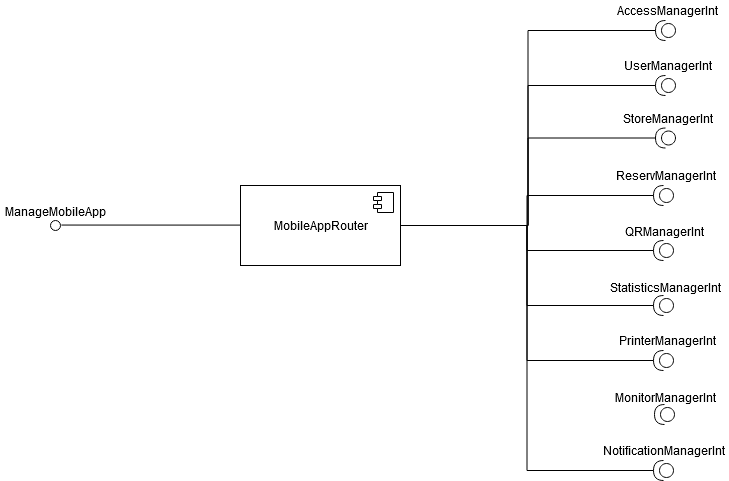
\includegraphics[scale=0.35]{Images/MobileAppRouting.png}
	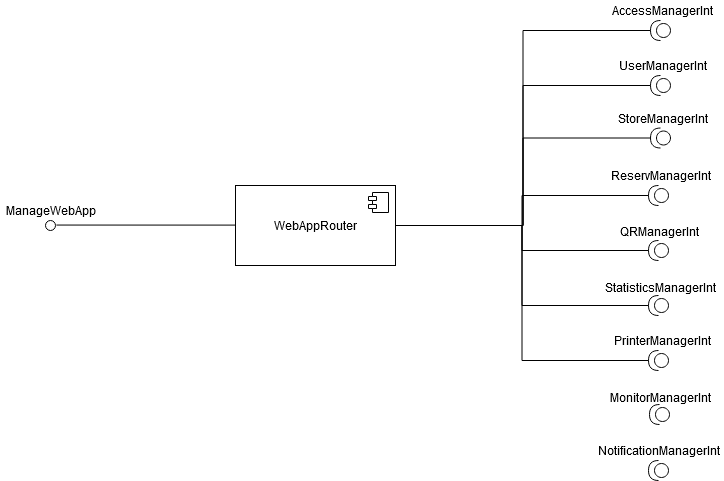
\includegraphics[scale=0.35]{Images/WebAppRouting.png}}
\end{figure}
\begin{figure}[H]
	\noindent
	\makebox[\textwidth]{
	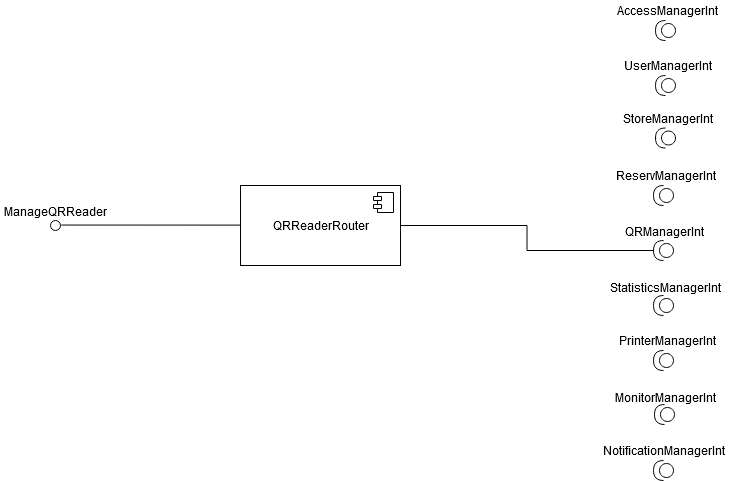
\includegraphics[scale=0.35]{Images/QRReaderRouting.png}
	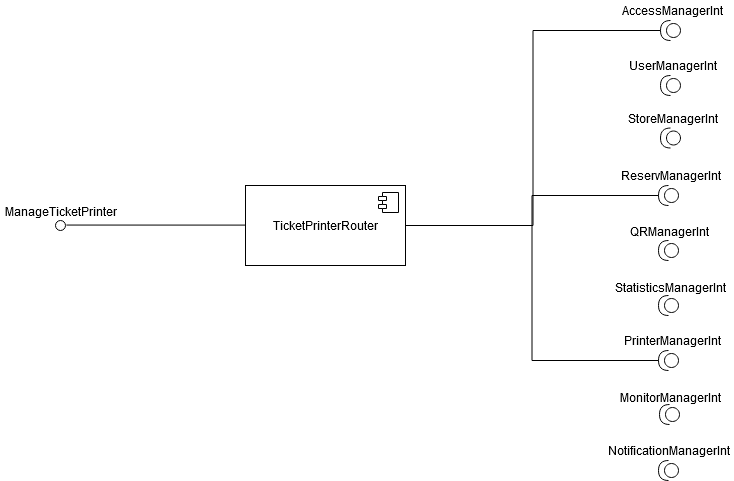
\includegraphics[scale=0.35]{Images/TicketPrinterRouting.png}}
\end{figure}
\begin{figure}[H]
	\noindent
	\makebox[\textwidth]{
	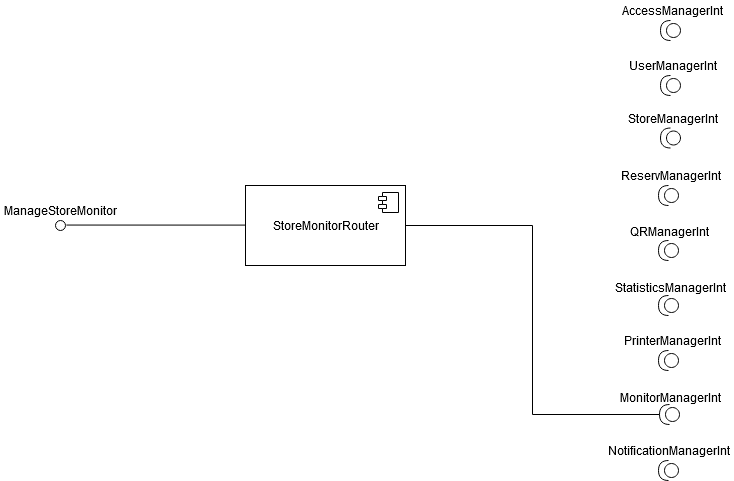
\includegraphics[scale=0.35]{Images/MonitorRouting.png}}
\end{figure}
\newpage
\subsection{Deployment View}
The following image shows the deployment diagram of the system by presenting the distribution (deployment) of software artifacts to the nodes, i.e. the deployment targets.
\begin{flushleft}
	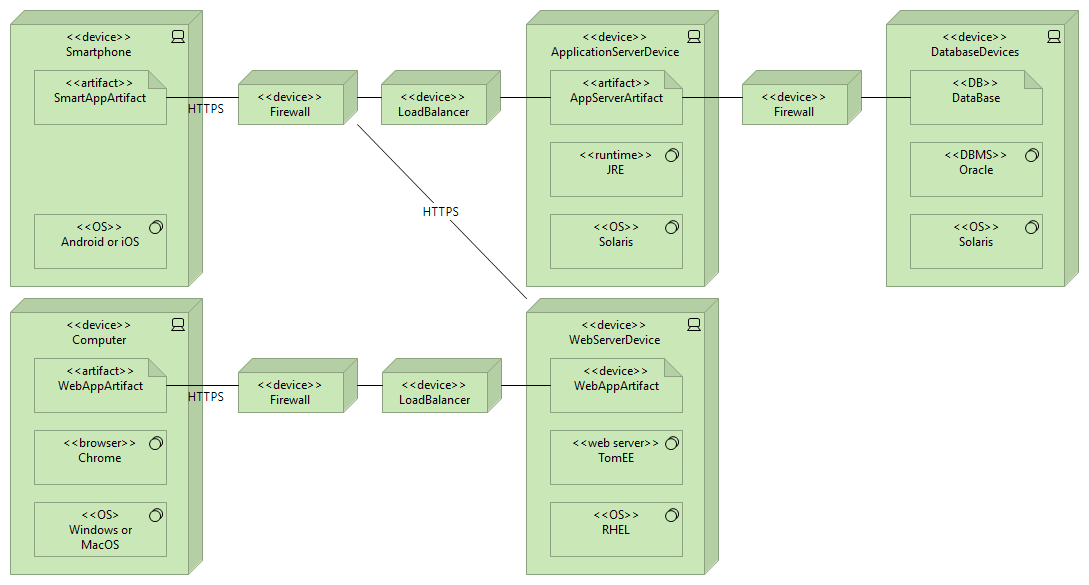
\includegraphics[scale=0.45]{Images/Deployment.png}
\end{flushleft}
Here we describe the components of the deployment view:
\subsubsection{Smartphone}
The customers and the store owners can access the functionalities of the system through a smartphone, that communicates through a firewall and a load balancer with the ApplicationServerDevice.\\
The SmartAppArtifact allows communication between the Smartphone and the ApplicationServerDevice, and its operation is supported by the operative system of the smartphone, either Android or iOS.
\subsubsection{Computer}
The customers and the store owners can access the functionalities of the system through a computer that communicates through a firewall and a load balancer with the WebServerDevice which in turn is connected through a firewall and a load balancer with an ApplicationServerDevice.\\
The WebAppArtifact will be downloaded from the WebServerDevice and it will be shown by the browser installed on the device which we assume for simplicity to be Chrome, whose operation is supported by the operating system of the Computer, either Windows or MacOs. 
\subsubsection{Firewall}
The firewalls allow to separate the different parts of the system: the DatabaseDevice is isolated from the ApplicationServerDevice, which in turn is isolated from the Smartphone, and the WebServerdevice, which in turn is isolated from the Computer.
\subsubsection{LoadBalancer}
The LoadBalancer allows to balance the load of the system on the replicated ApplicationServerDevices and WebServerDevices.
\subsubsection{ApplicationServerDevice}
This device implements the main business logic of our system. It is accessed by Smartphone and Computer devices to make use of the functionalities offered by the system. It is supported by a DatabaseDevice that allows the ApplicationDevice to create, read, update and delete all the information necessary for the correct functioning of the system.\\
The AppServerArtifact is run by the JRE which in turn is supported by the RHEL operating system.
\subsubsection{WebServerDevice}
This device allows customers and store owners to access their respective services by using Java RMI to communicate with the ApplicationServerDevice.\\
The web server TomEE will server the browser the artifact it needs to show to the users. This web server's operation will be supported by Red Hat Linux Enterprise operating system.
\subsubsection{DatabaseDevice}
This device allows the ApplicationServerDevice to create, read, update, delete information that supports the system operation.\\
The DataBase is managed by the Oracle DBMS which in turn is supported by Oracle Solaris.\newpage
\subsection{Runtime View}
%TODO : something here
\subsubsection{Login via smartphone app}
\begin{figure}[H]
	\noindent
	\makebox[\textwidth]{
	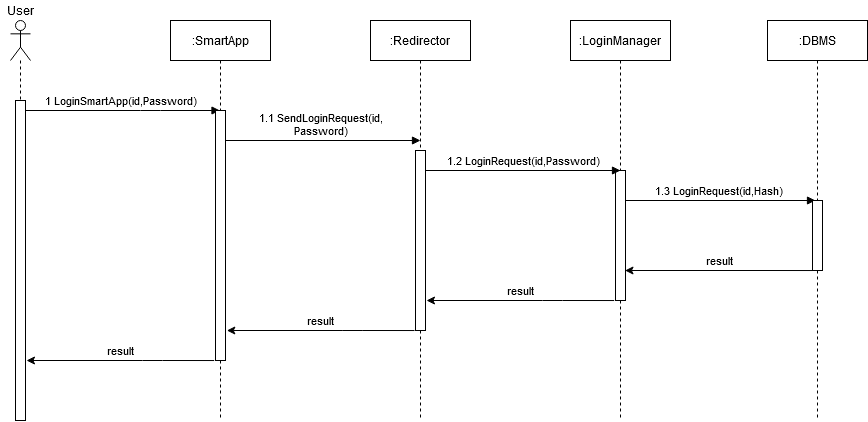
\includegraphics[scale=0.5]{Images/RuntimeViewLogin.png}}
\end{figure}
%TODO : dashed arrows on responses
By opening the application, user calls the SmartApp component. SmartApp calls Redirector, that calls LoginManager, that retrieves from the DBMS the password hash of the specified user (if he/she exists), and compares it with the provided password. The result of this operation is then sent back to the user.\\
\subsubsection{Immediate reservation via smartphone app}
\begin{figure}[H]
	\noindent
	\makebox[\textwidth]{
	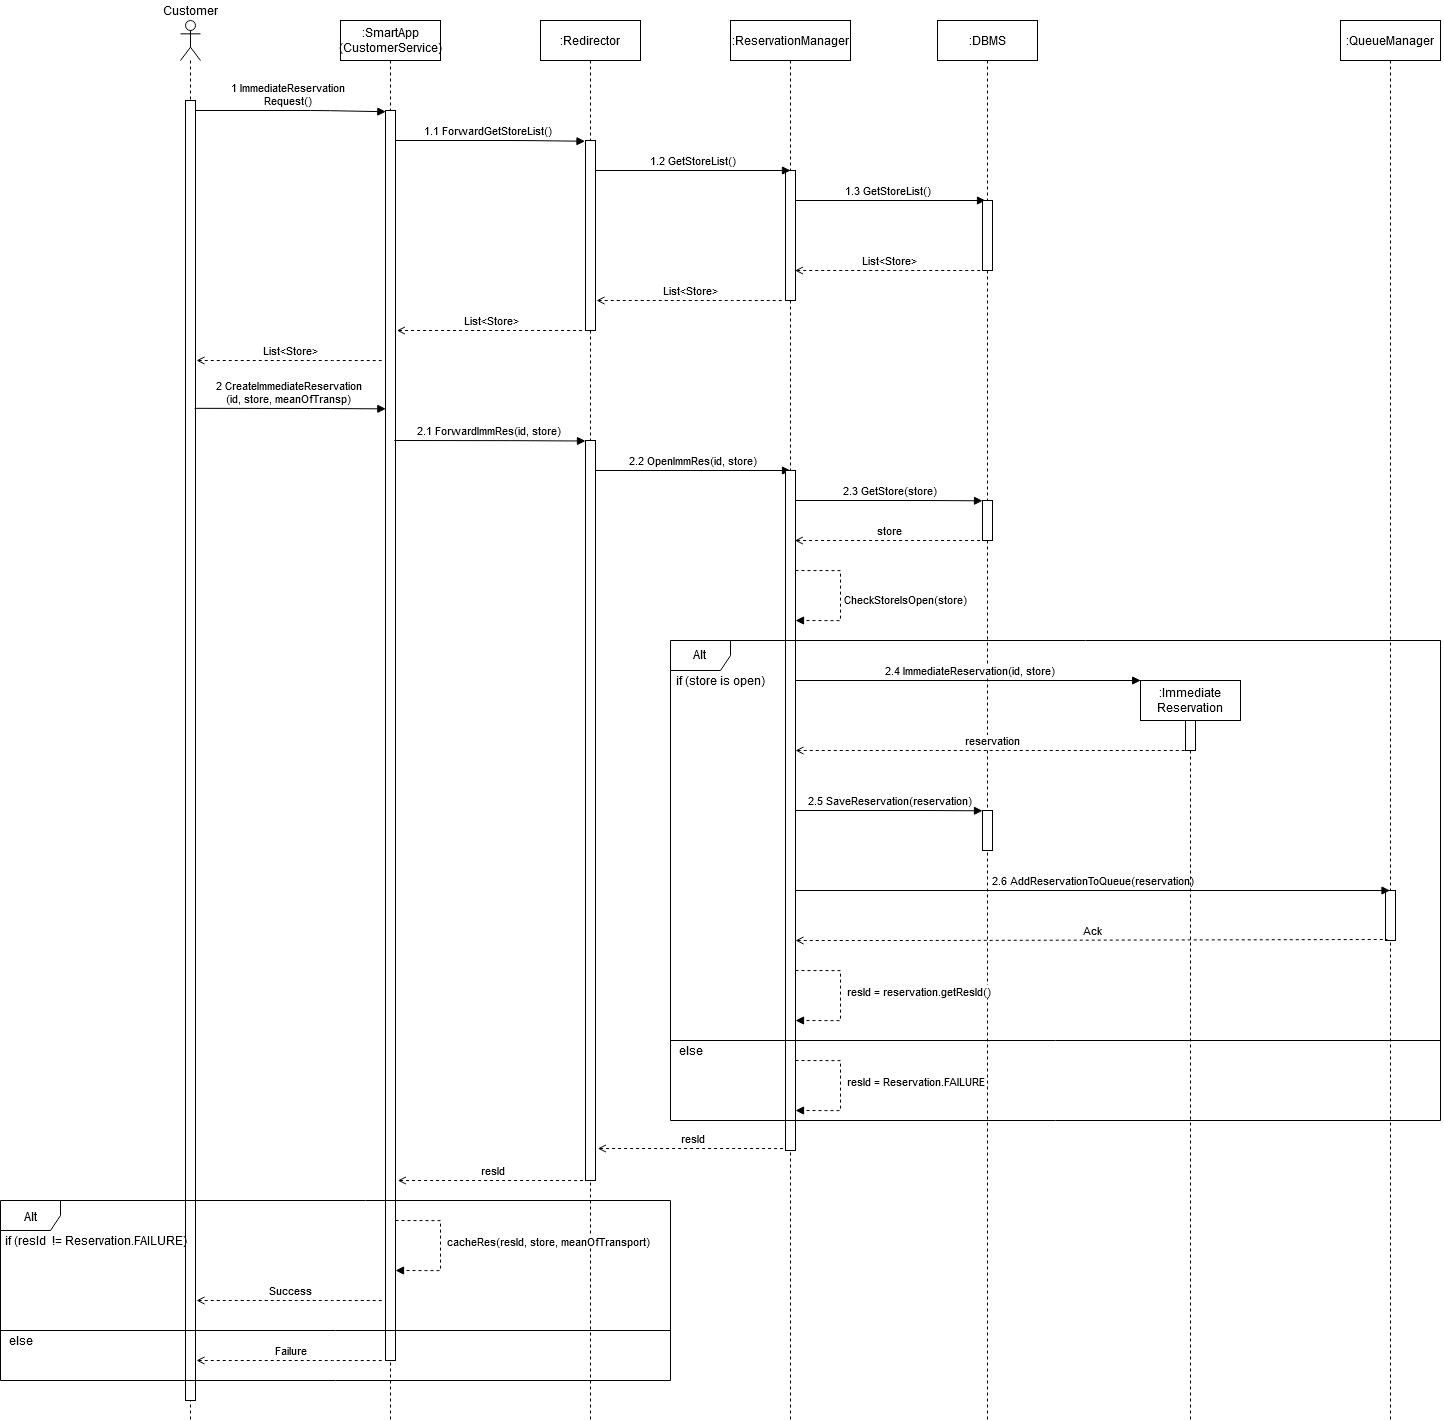
\includegraphics[scale=0.35]{Images/RuntimeViewImmRes.png}}
\end{figure}
The customer selects the option to create an immediate reservation. The SmartApp requests a list of stores from the ApplicationServer and this request is then forwarded by the Redirector to the ReservationManager that retrieves the list of stores form the DMBS and sends it back to the customer. The customer then selects a store form the list provided and a means of transport. This information is then sent to the ApplicationServer where the Redirector routes it to the ReservationManager that checks that the selected store is open at the time, loading it from the DBMS, and if it is, the reservation is confirmed, added to the queue of that store by calling QueueManager, and saved in the DBMS. It is rejected otherwise.
\subsubsection{Future reservation via web app}
\begin{figure}[H]
	\noindent
	\makebox[\textwidth]{
		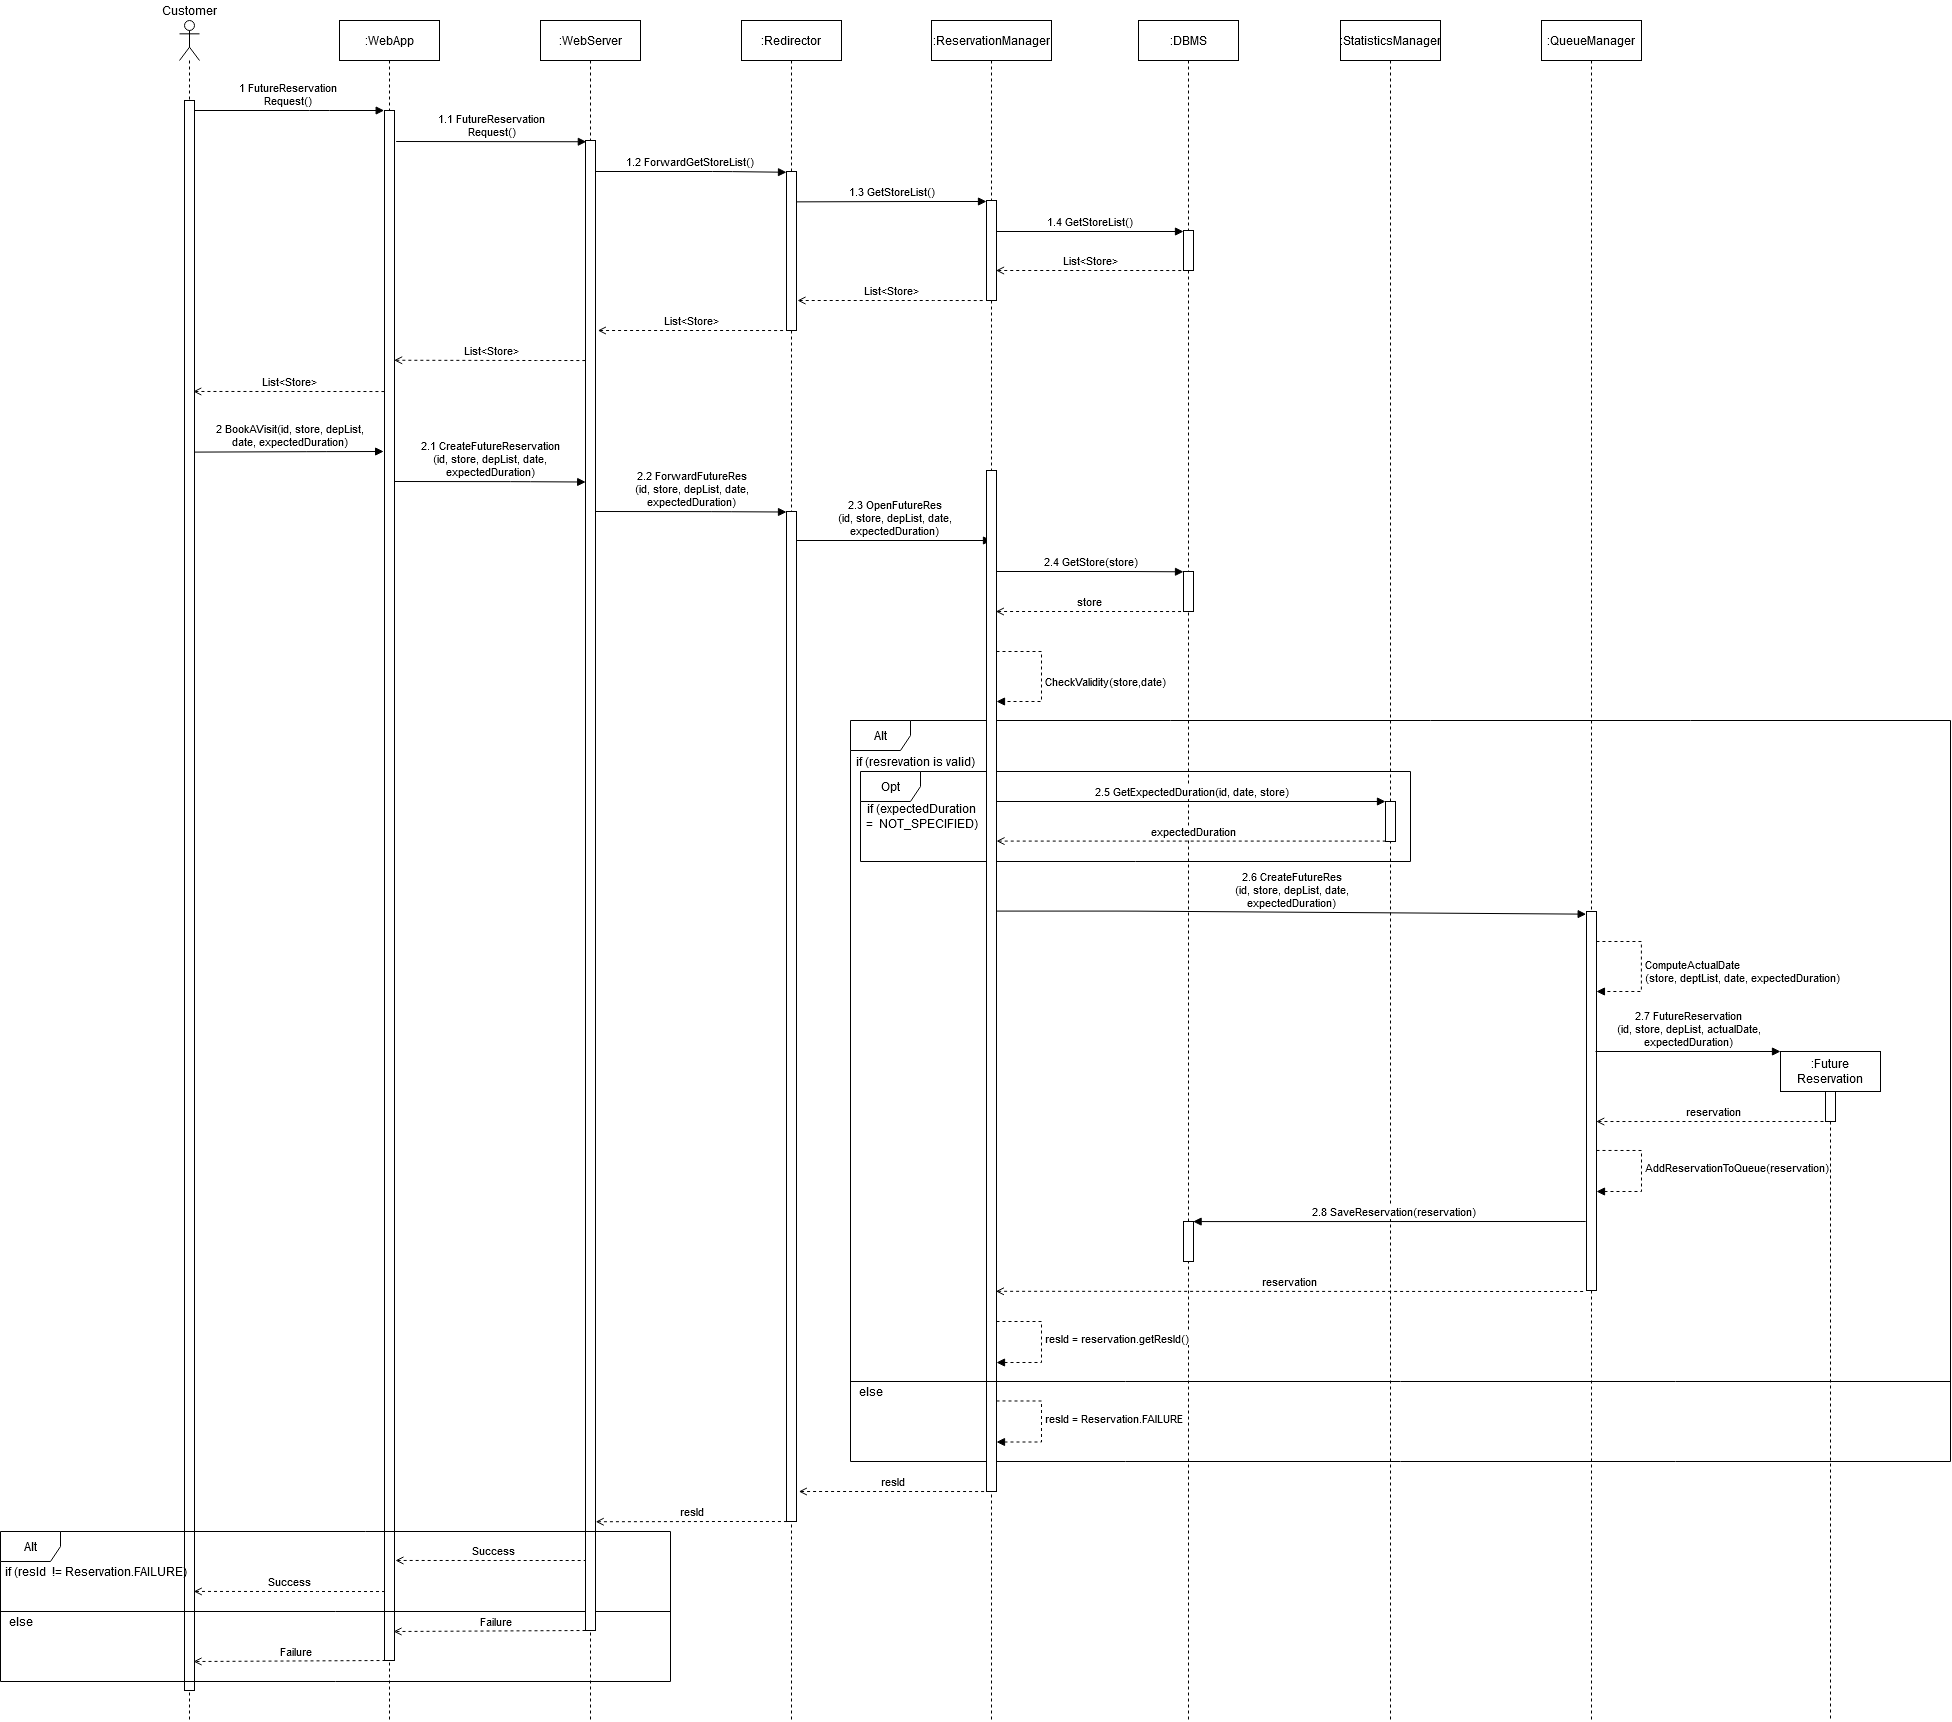
\includegraphics[scale=0.3]{Images/RuntimeViewFutRes.png}}
\end{figure}
When the customer selects the option to book a visit, the WebApp, through the WebServer, requests a list of stores from the ApplicationServer and this request is then forwarded by the Redirector to the ReservationManager that retrieves the list of stores form the DMBS and sends it back to the customer.\\
The customer can then select a store form the list provided, the date he would like to book and, optionally, a list of departments he is interested in and how long he thinks the visit will be. This information is then sent to the ApplicationServer where the Redirector routes it to the ReservationManager that checks that the resrvation is valid (the selected store is open at the time, the maximum number of reservations has not yet been reached), and if it is, the reservation can be generated: first, if the expected duration has not been specified, it is inferred by the StatisticsManager, based on the past reservations created by the customer, and returned to the ReservationManager; then it ask the queue manager to create the reservation and insert it into the queue in an appropriate time slot, considering the other reservations already present. The reservation is then saved into the DBMS.\\
If the reservation was not valid, then it is rejected.
\subsubsection{On premise reservation}
\begin{figure}[H]
	\noindent
	\makebox[\textwidth]{
		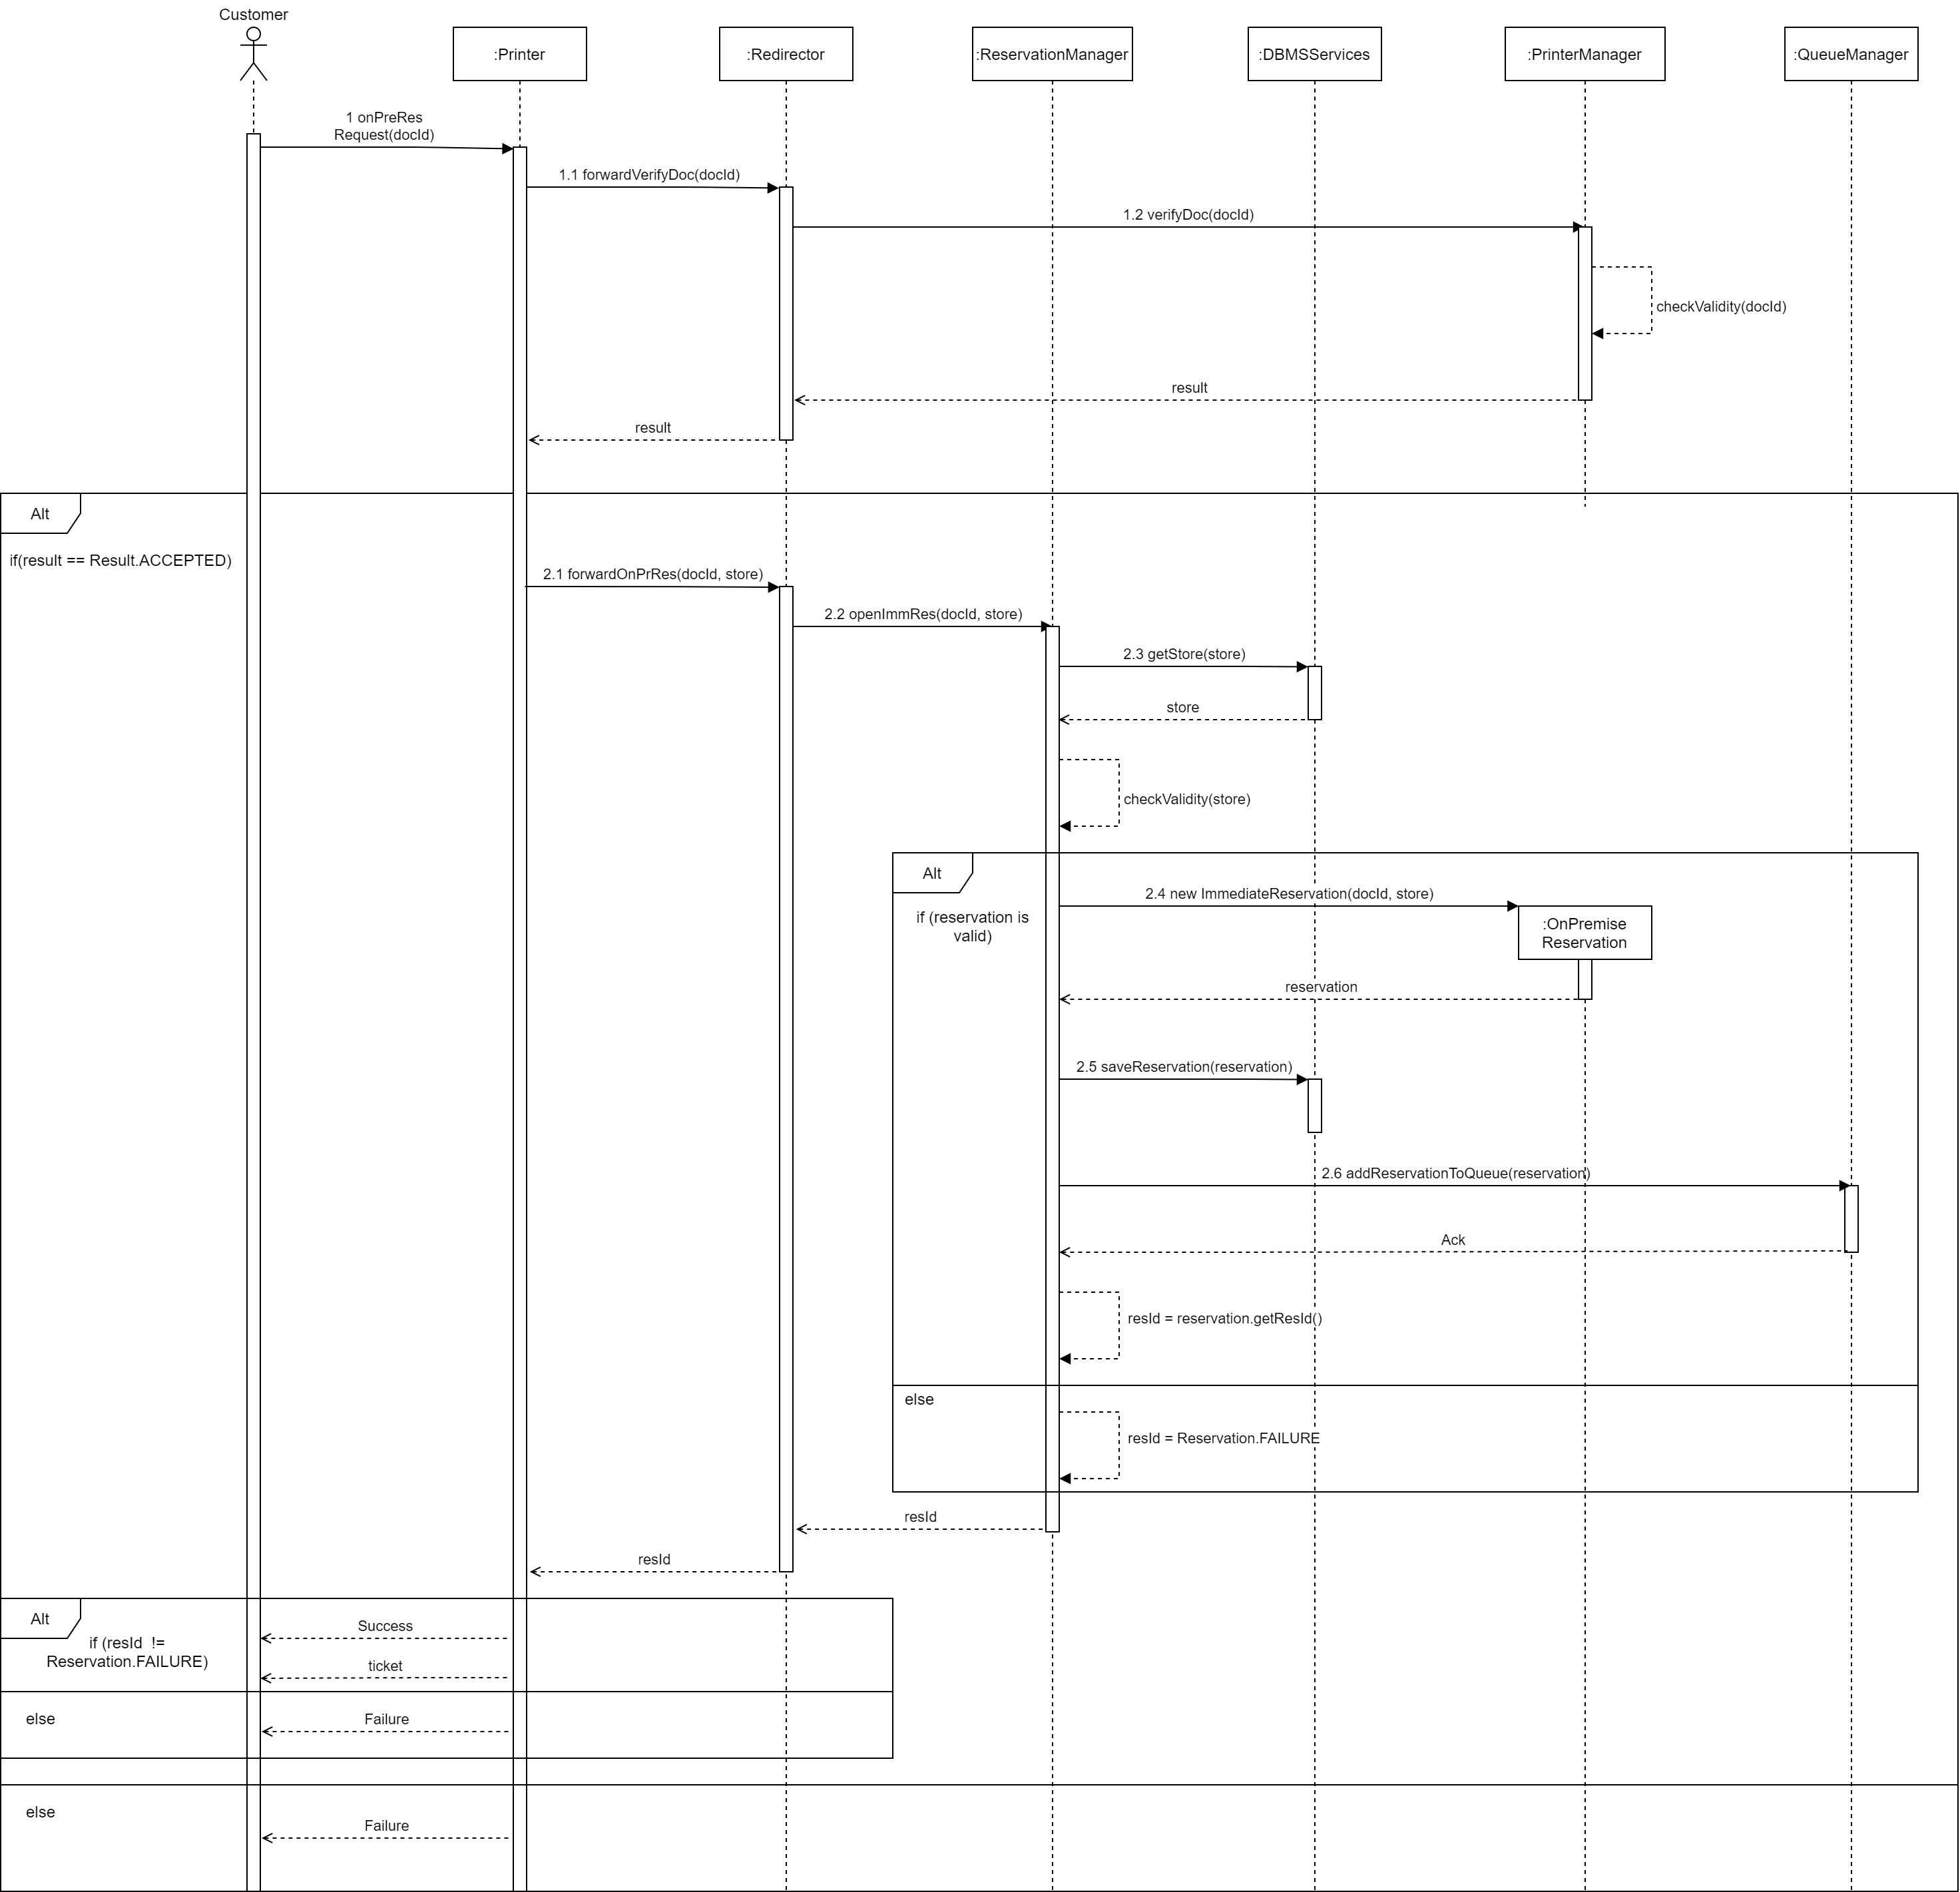
\includegraphics[scale=0.35]{Images/RuntimeViewPreRes.png}}
\end{figure}
The customer selects the option to create an on premise reservation, and provides the TicketPrinter with an identification document. This request is then forwarded by the Redirector to the PrinterManager that checks that the document is valid. If it is, an on premise reservation request is then sent to the ApplicationServer where the Redirector routes it to the ReservationManager that checks that that the reservation is valid for the selected store at the time of creation (e.g. the store is open), loading the store info from the DBMS, and if it is, the reservation is confirmed, added to the queue of that store by calling QueueManager, and saved in the DBMS. It is rejected otherwise.
\subsubsection{Statistics generation}
\begin{figure}[H]
	\noindent
	\makebox[\textwidth]{
	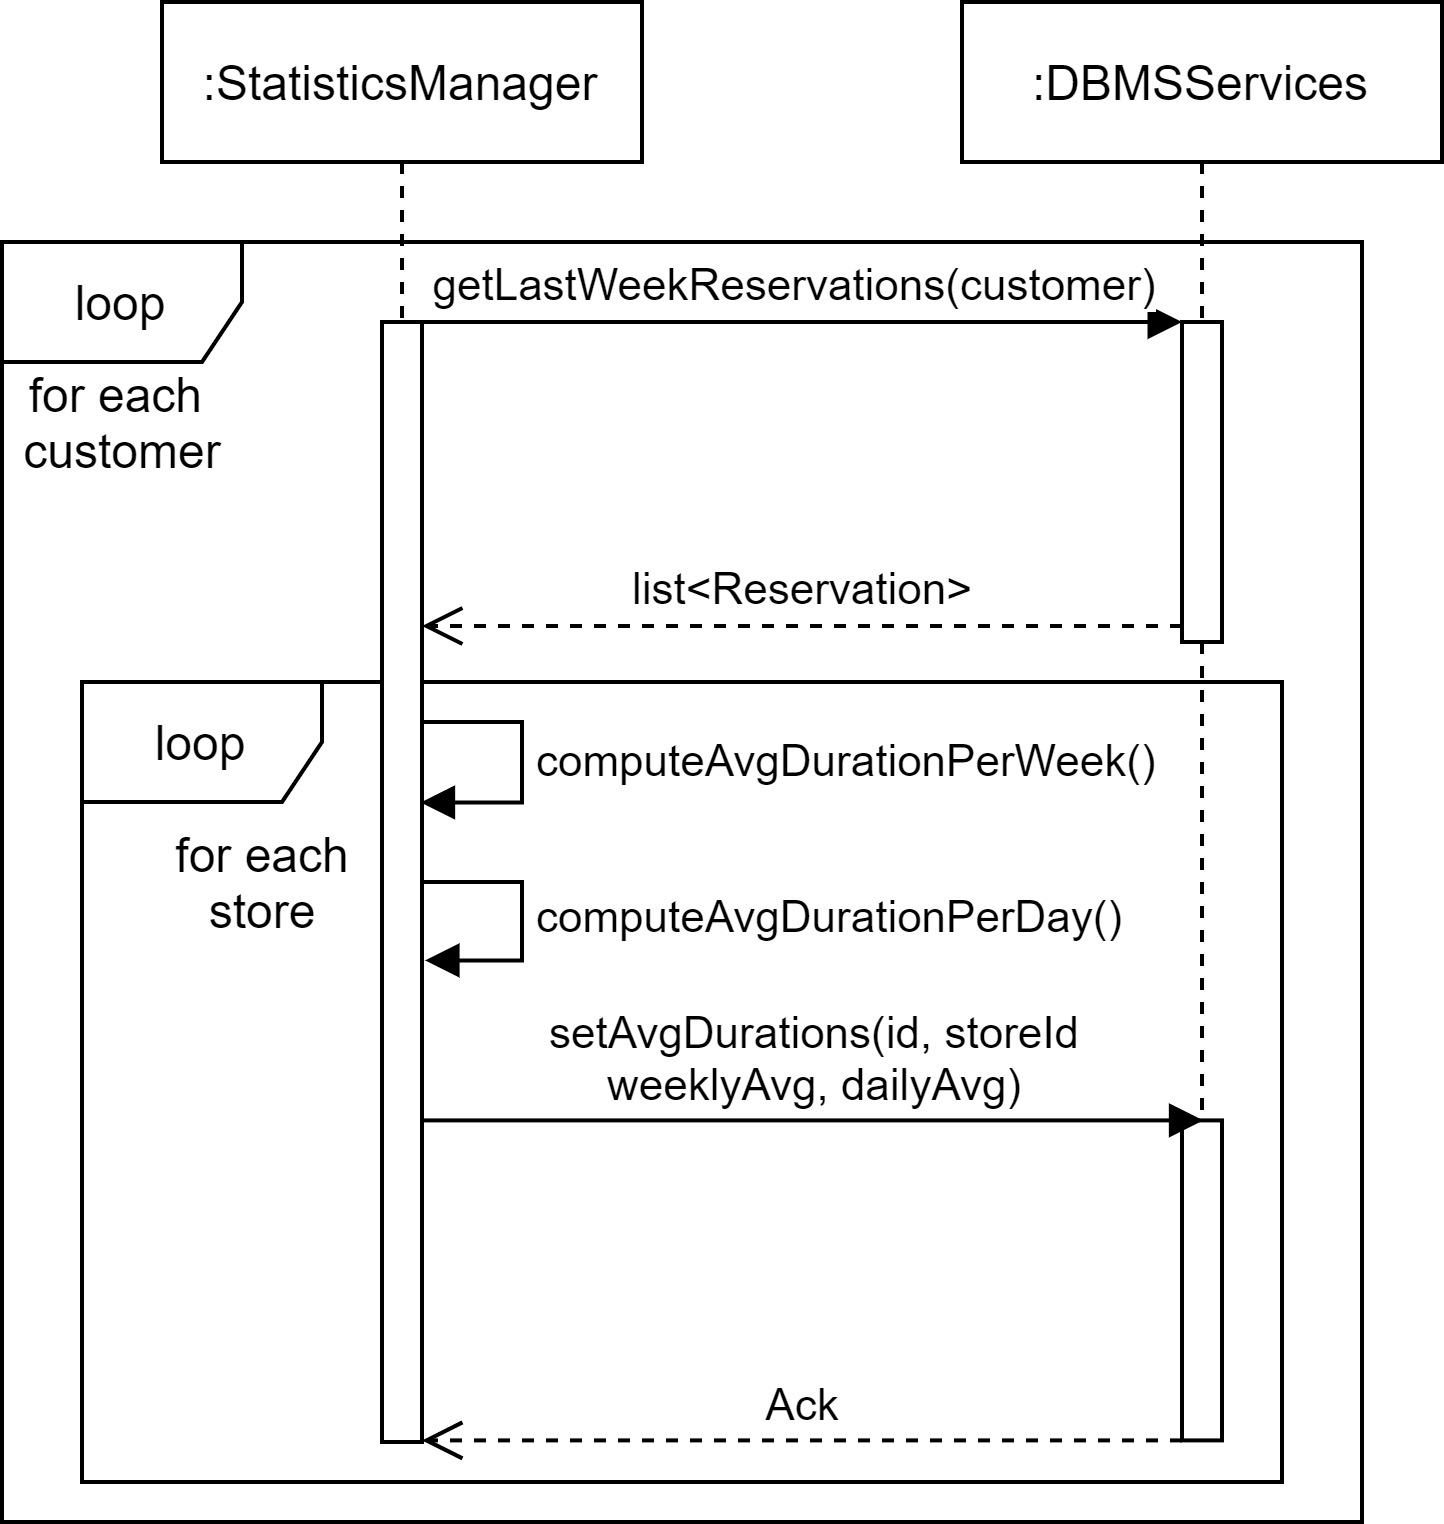
\includegraphics[scale=0.5]{Images/RuntimeViewStatistics.png}}
\end{figure}
Every week the StatisticsManager retrieves a list of the reservations of the past week, and for each customer and each store computes the average daily and weekly duration of the visit, and stores them in the DBMS.
\subsubsection{Customer enters store}
\begin{figure}[H]
	\noindent
	\makebox[\textwidth]{
	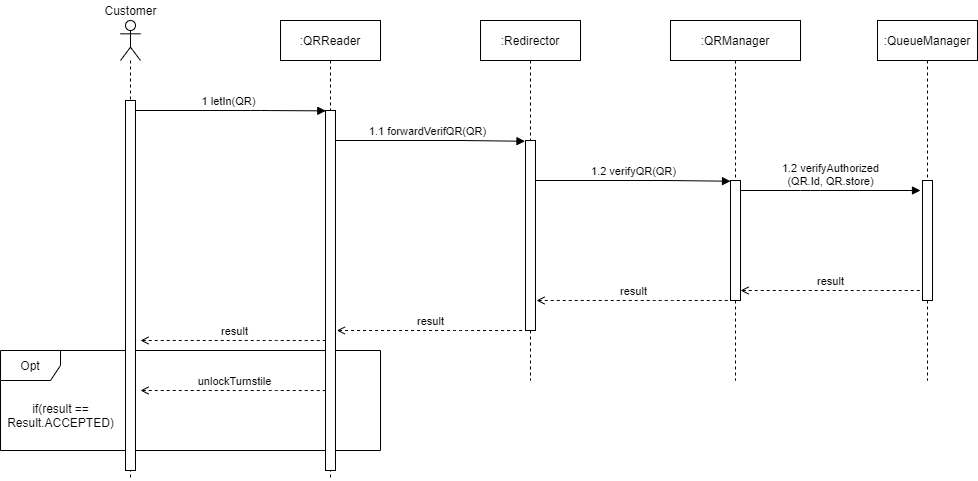
\includegraphics[scale=0.45]{Images/RuntimeViewStoreEntry.png}}
\end{figure}
The customer provides the QR reader with a QR code (be it on the screen of his/her smartphone or printed on paper). That code is then forwarded by the redirector to the QRManager that decodes it and calls the QueueManager to check that the QR code belongs to a customer that is now authorized to enter the store. If this is the case, the turnstiles unlock. Whenever the customer enters or exits a store, QueueManager saves the time of arrival/departure in the reservation, and then saves them in the DBMS.
\subsubsection{Store owner registers store via web app}
\begin{figure}[H]
	\noindent
	\makebox[\textwidth]{
	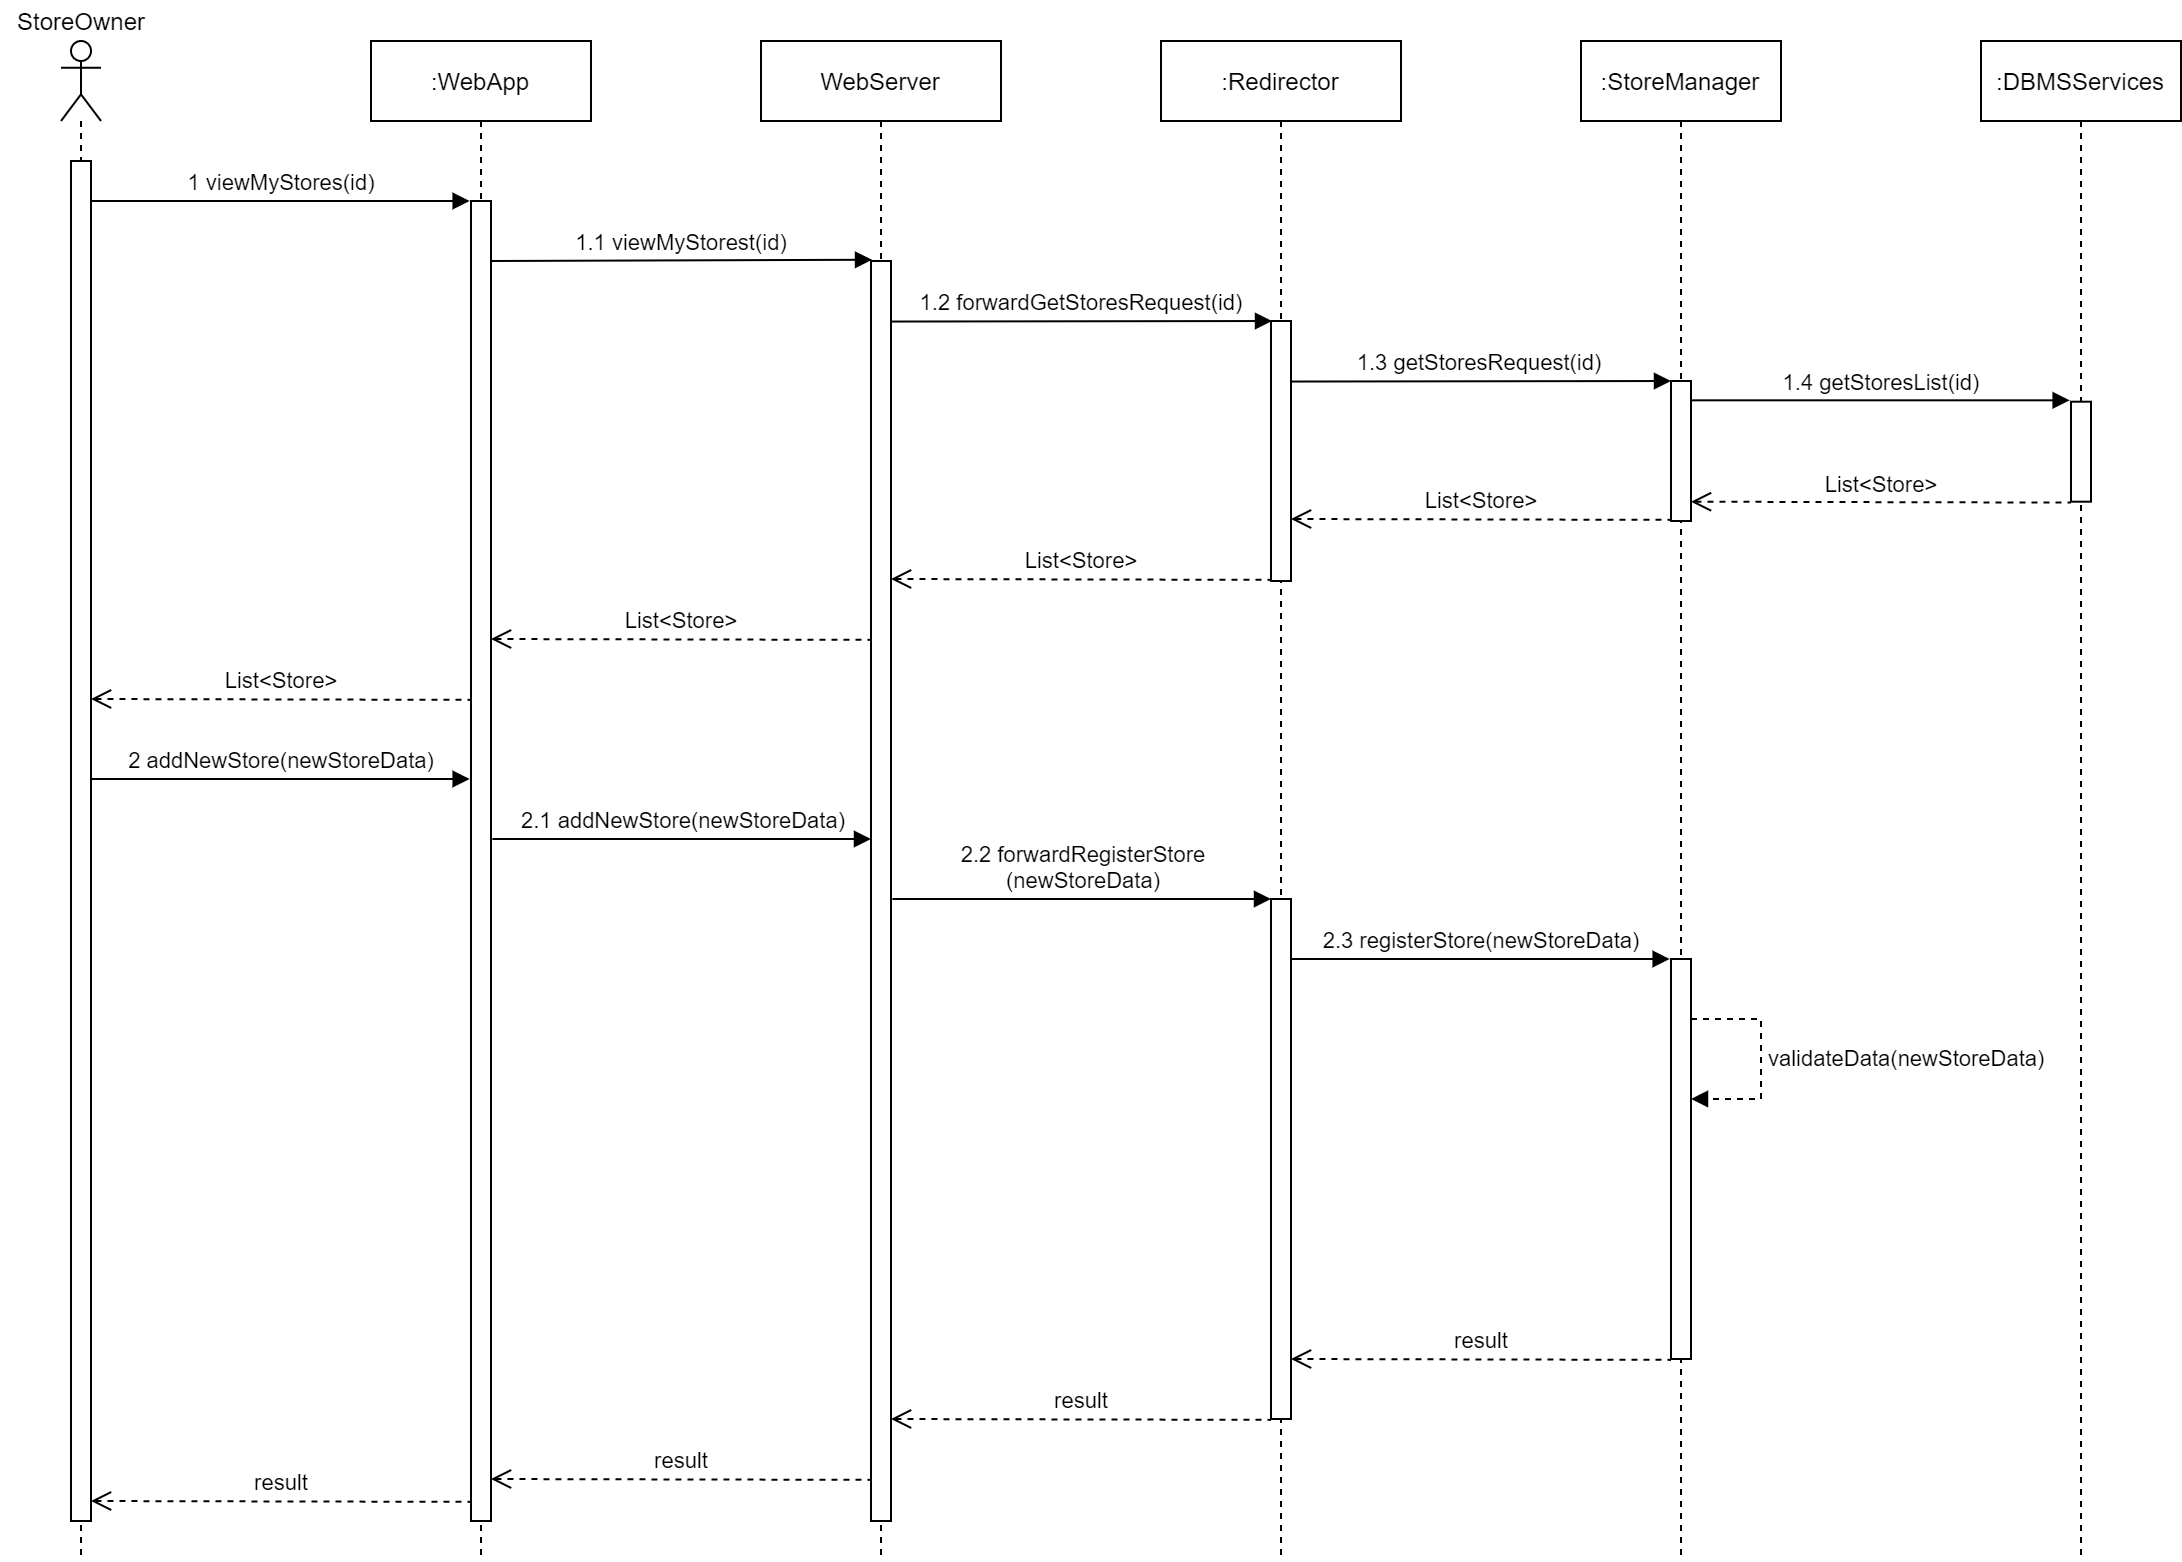
\includegraphics[scale=0.35]{Images/RuntimeViewStoreReg.png}}
\end{figure}
The store owner opens the app and look at all his/her stores; he/she decides to add a new store, so he/she insert all required data, that are sent, through the redirector, to the StoreManager. This component validates the data and, if everything is correct, asks the DBMS to save the data of the new store.\\
Of course, in this process, only the store has been added, so the store owner will then also need to register the TicketPrinter, the QRReader and the StoreMonitor to the system.
\subsubsection{Customer is notified by smartphone app}
\begin{figure}[H]
	\noindent
	\makebox[\textwidth]{
	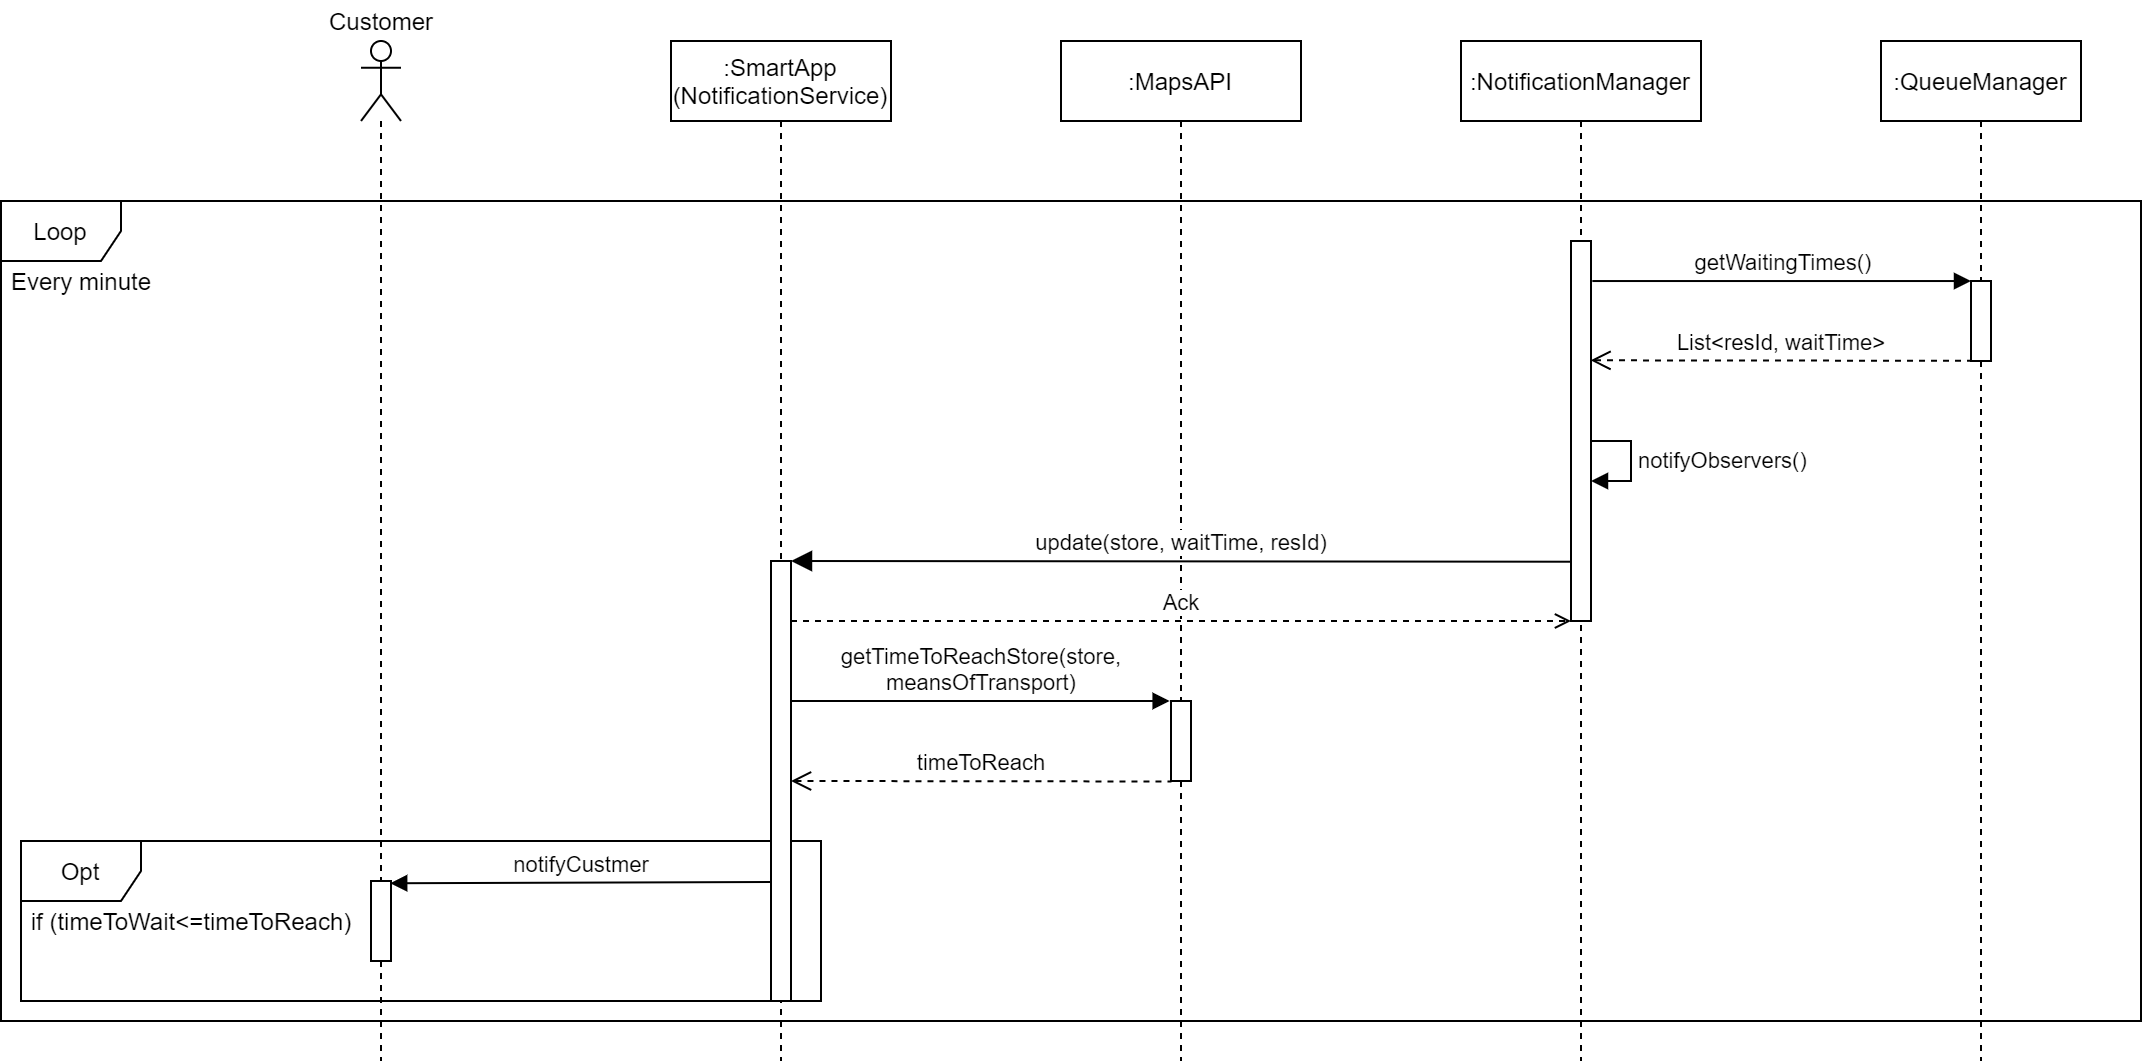
\includegraphics[scale=0.35]{Images/RuntimeViewNotification.png}}
\end{figure}
Periodically the system must check if it is time to notify the customer about his/her reservations.\\
Once every minute, the NotificationManager will ask the QueueManager to send, for each of the relatively closest reservations(those that hava as target time less than an hour with respact to the current time) the time remaining before they become authorized. Each of this times is then sent to its respective customer, if the reservation has been generated by a phone app.\\
Then the phone app will use the MapAPI to get an estimation of the time necessary to reach the store from the location of the device, by the means of transport specified at the creation of the reservation. Now, by comparing this two numbers, it can decide whether notify the customer or not. Of course there can actually be an additional value n such that the customer is notified if time to wait <= time to reach + n. In this way the customer has a little notice before departing.
\newpage
\subsection{Component Interfaces}
\begin{figure}[H]
	\noindent
	\makebox[\textwidth]{
	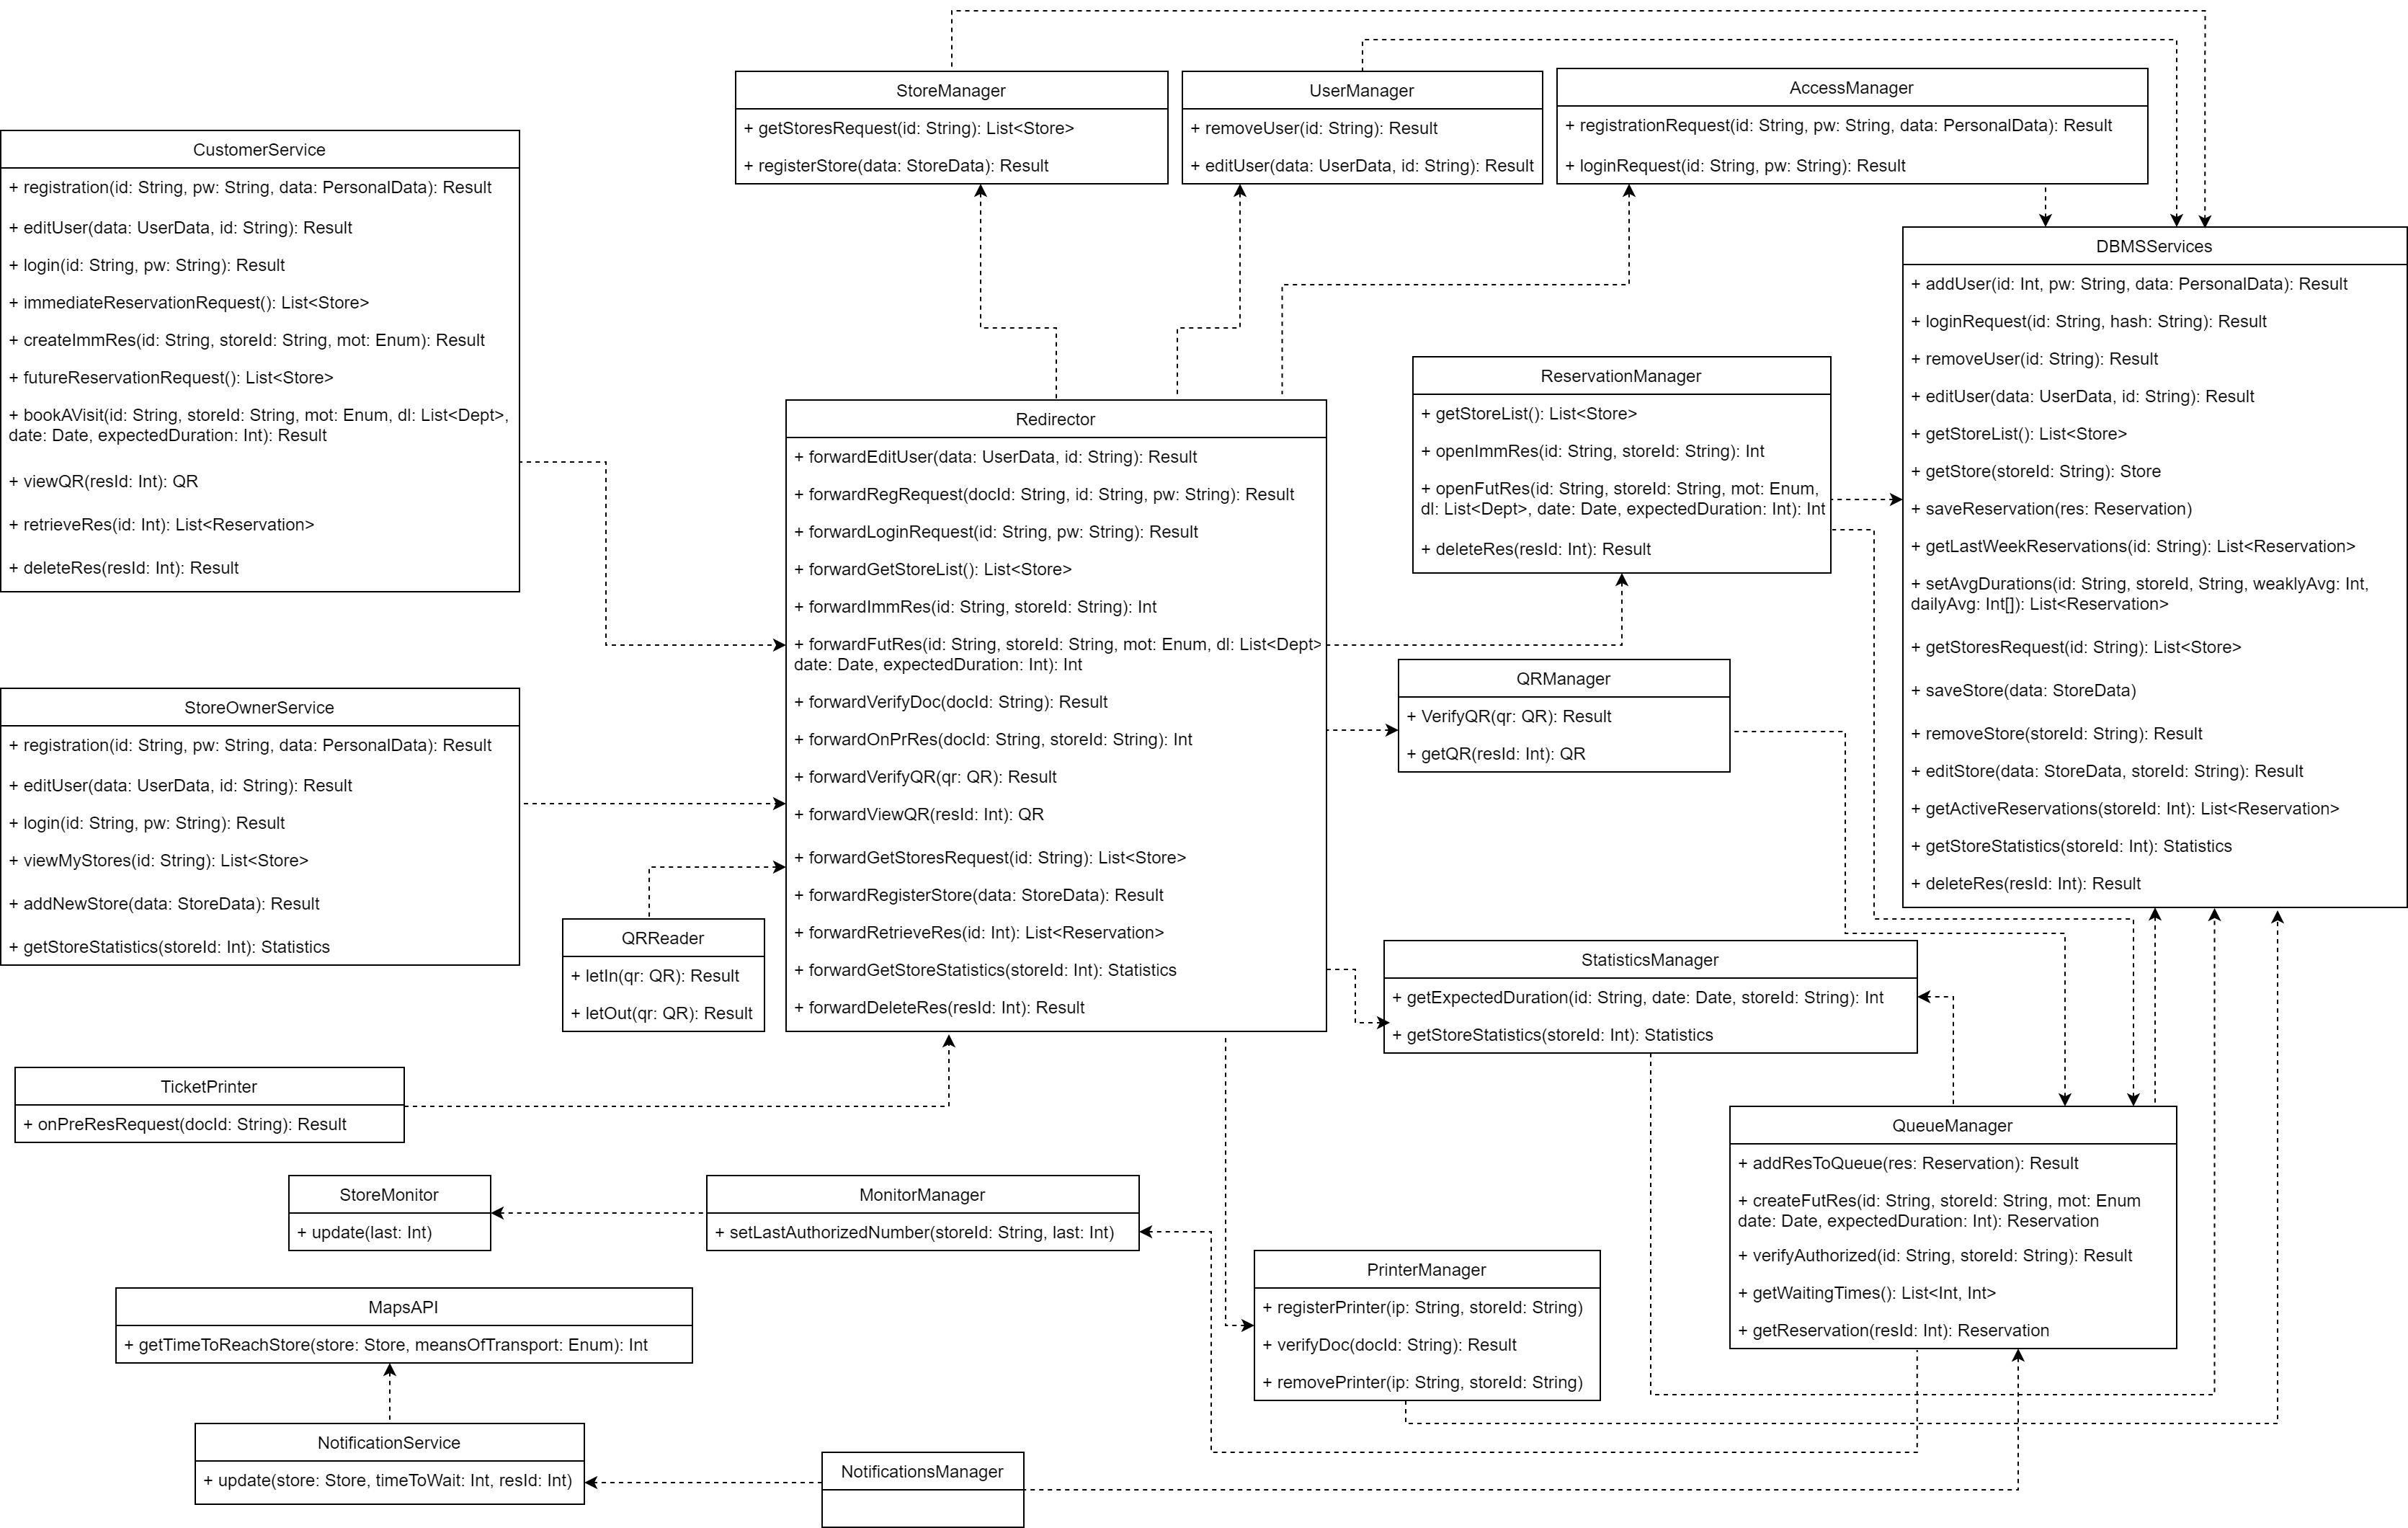
\includegraphics[scale=0.45]{Images/ComponentInterfaces.png}}
	\caption{Component Interfaces} %TODO: decide wether to keep captions
\end{figure}
In this diagram we represented the interfaces of the system components with their methods, and such interfaces interact with each other.\\
For ease of representation we split WebApp and SmartApp component functionalities into three interfaces: CustomerService, StoreOwnerService and NotificationService. The WebApp component, that allows customers and store owners to interact with the system with a computer, implements the CustomerService and the StoreOwnerService interfaces. The SmartApp component, that allows customers and store owners to interact with the system with a smartphone, implements the CustomerService, StoreOwnerService and NotificationService interfaces.\\\\
All communication from the outside world (except DBMS) to the ApplicationServer is mediated by the Redirector, while the ApplicationServer sends messages directly to the interested components: NotificationService communicates directly with the NotificationService, and MonitorManager communicates directly with the StoreMonitor component.\\
Methods written here provide a logical representation of what component interfaces have to offer. They will be a soft guideline for the developers, that will be able to adapt them to create working components, facing the various problems that emerge during the implementation.\\
At time of creation a user is assigned a string called id that uniquely represents that user. At time of creation a reservation is assigned a string called resId that uniquely represents it.\\
\subsection{Selected Architectural Style and Patterns}
The proposed architecture of the system make use of several architectural patterns, some of which has already been breafly described in the previous sections. We now present a more expanded specification of those architectural choices.\\\\
\subsubsection{Three layer Client-Server}
The overall architecture is a Three layer (presentation, application, data) client-server structure. This pattern has already been previously detailed, so check Section 2.1: Overview for more information about this style and why it has been chosen.
\subsubsection{RESTful architecture}
To manage the distributed system we choose a Representational state transfer (REST) architectural style. This style provides a data transmission system based on HTTP, with no other layers, which creates a stateless communication, i.e. it doesn't support the existence of sessions. In the RESTful Web Service requests are made to the URL of the resource or of the set of resources, which must be well defined and unambiguous. All operations will be mapped to the HTTP methods, e.g. GET, POST, PUT, DELETE.\\\\ This architectural style is used for fast performance, due to the absence of coupling between client and server components and upper layers to the HTTP protocol, and to ensure the ability to grow, by reusing components that can be managed and updated without affecting the system as a whole. In fact, due to the pandemic, the S2B has a strict time to market that we need to hit, in order to provide our functionalities when they are more needed; for this reason every extra function or modification we may want to add will need to be implemented after the release of the application, so an easy to update architecture is highly advised.\\\\
As a REST architecture the system will support cacheability, eliminating some client–server interactions, further improving scalability and performance.\\
Moreover it must have a single uniform interface, that simplifies and decouples the architecture, which enables each part to evolve independently. This constraint is checked by its subconstraints:
\begin{itemize}
	\item in our system resources identified in requests are conceptually separate from the representations that are returned to the client
	\item resources given to the client can be manipulated through the client representation
	\item each message includes enough information to describe how to process the message
	\item the client is able from the initial URL to use server-provided links dynamically to discover all the available resources it needs
\end{itemize}
The other constraint of the REST style, i.e. the layered system with client-server architecture, has already been discussed in the previous sections of this document. 